\documentclass[11pt,a4paper]{article}
\usepackage[margin=25mm]{geometry}
\usepackage[T1]{fontenc}
\usepackage[utf8]{inputenc}
\usepackage{lmodern,microtype}
\usepackage{amsmath,amssymb,amsthm,mathtools}
\usepackage{booktabs,longtable,tabularx,array}
\usepackage{enumitem,xcolor,graphicx}
\usepackage{listings}
\usepackage[colorlinks=true,linkcolor=blue!45!black,citecolor=teal!50!black,urlcolor=blue!50!black]{hyperref}
\usepackage{fancyhdr}
\definecolor{ink}{RGB}{25,47,68}
\definecolor{teal}{RGB}{0,111,117}
\pagestyle{fancy}\fancyhf{}
\fancyhead[L]{\small\color{ink}Native compressed topology for unknot recognition}
\fancyhead[R]{\small 8 October 2026}
\fancyfoot[C]{\thepage}
\setlength{\headheight}{14pt}
\raggedbottom
\setlength{\parindent}{0pt}\setlength{\parskip}{5pt}
\setlist{nosep,leftmargin=*}
\newtheorem{theorem}{Theorem}[section]
\newtheorem{proposition}[theorem]{Proposition}
\newtheorem{lemma}[theorem]{Lemma}
\newtheorem{corollary}[theorem]{Corollary}
\theoremstyle{definition}\newtheorem{definition}[theorem]{Definition}
\theoremstyle{remark}\newtheorem{remark}[theorem]{Remark}
\newcommand{\F}{\mathbb F_2}
\newcommand{\bits}{\operatorname{bits}}
\newcommand{\cl}{\operatorname{cl}}
\newcommand{\orb}{\operatorname{orb}}
\newcommand{\code}[1]{\texttt{#1}}
\newcommand{\poly}{\operatorname{poly}}
\newcommand{\qp}{n^{O(\log n)}}
\lstset{basicstyle=\ttfamily\footnotesize,breaklines=true,columns=fullflexible,
  keepspaces=true,frame=single,rulecolor=\color{black!15},backgroundcolor=\color{black!2},
  aboveskip=9pt,belowskip=9pt,showstringspaces=false}
\hypersetup{pdftitle={General interval orbits, native normal-surface certificates, and sparse meridian search},
  pdfauthor={Research continuation prepared with ChatGPT for ProveIt}}
\title{\color{ink}Toward Quasi-Polynomial Unknot Recognition\\[5pt]
  \Large General Interval Orbits, Native Normal-Surface Certificates,\\
  Port Incidence, and Sparse Meridian Search}
\author{Research continuation for the ProveIt project\\
  \small Prepared with ChatGPT: algorithms, proofs, implementation, and experiments}
\date{8 October 2026}

\begin{document}
\maketitle
\begin{abstract}
The preceding research produced compressed normal-disc identifications but
left them without a general native consumer. We close that implementation gap
by independently implementing the Agol--Hass--Thurston orbit-counting
algorithm for arbitrary partial translations and reflections of a binary-sized
integer interval. A separate checker verifies local reduction traces without
running the producer's scheduling algorithm. We connect this engine to the
existing normal-coordinate extractor, obtaining exact component counts,
orientability counts, boundary counts, Euler characteristic, and a native
certificate for a supplied normal compressing disc. None of these operations
enumerates the represented normal discs.

A coning identity reduces marked-component incidence to ordinary orbit counts.
Boolean M\"obius inversion then recovers the complete histogram of attachment
signatures for $r$ marked sets in $2^r\poly(k+m+r,B)$ time, where $k$ is the number
of input pairings, $m$ the number of marked intervals, and $B$ their bit size.
This is a precise parameterized query theorem, including a quasi-polynomial
regime, rather than an assertion that the full geometry of attachments is known.

Separately, we prove that a binary implication system with trivial singleton
closures needs to test only its distinct two-element prerequisite sets when
searching for two generators. For the checked Wirtinger systems this leaves at
most $2n$ candidate pairs. Generation-stamped propagation and closed-set
pruning avoid repeatedly initializing the entire system. The optimized search
preserves the first successful seeds, derivation order, and existing positive
certificates. We validate the new components against literal finite oracles,
the previous implementation, and Regina, and report paired performance with
its actual scope.

The general $\qp$ recognition theorem is \emph{not established}. The remaining
obligations include finding suitable normal surfaces, completing attachment-aware
cutting, and bounding intermediate encoded size, hierarchy depth and resets.
The contribution is a working general compression bridge and a proved sparse
search improvement, with explicit boundaries between classical mathematics,
new derived queries, verified code, and open research.
\end{abstract}
\clearpage
\setcounter{tocdepth}{1}
\tableofcontents
\clearpage

\section{Outcome, baseline, and attribution}
\label{sec:outcome}

The implementation baseline is commit
\begin{center}\small\texttt{2b93767bd3cf7ea7c1995acd66f50c72858a30c5}\end{center}
of \href{https://github.com/VladimirReshetnikov/ProveIt}{VladimirReshetnikov/ProveIt},
under \path{Topology/UnknotRecognition}. The GitHub connector was used to inspect
the maintained project, and a sparse checkout of this exact revision was used
for development and comparisons. The checkout is pinned even if the remote
branch changes while experiments run. The delivered patch targets this revision;
the accompanying runnable snapshot avoids dependence on a moving branch.

Independent checks in this report use distinct implementations or
representations. The mathematical arguments and executable certificate
checkers have not undergone external peer review or proof-assistant
formalization.

The distinction between the latest maintained code and earlier reports is
material. The main README contains historical test counts and integration
checkpoints. We instead inspected the current modules and the synthesis review
of the incoming affine-families archive. That review explicitly identifies the
missing native consumer of its partial signed interval maps. Its affine-family
optimizer operates on total cyclic translations; those hypotheses cannot simply
be imposed on the normal-coordinate maps.

\begin{center}\small
\begin{tabularx}{\textwidth}{@{}p{.22\textwidth}XX@{}}
\toprule
Object & Prior status & This continuation\\\midrule
Normal-disc face bands & Extracted in the preceding affine-families report;
only small explicit and external-native consumers & Prior extractor imported
unchanged, with its tests and attribution\\
General interval orbits & Classical AHT theorem; no maintained native engine &
Independent producer, separate trace checker, arbitrary partial isometries\\
Normal surface topology & Compressed input prepared; full sheet expansion
avoided only by an external engine & Native aggregate topology and supplied-disc
certificate, with explicit ambient preconditions\\
Marked attachments & Special cyclic/dihedral formulas and unresolved arbitrary
partial-map bridge & Exact orbit-incidence histogram by coning and M\"obius
inversion; cyclic order and attaching words remain outside its scope\\
Two-meridian seed search & Dense setup for each lexicographically tested seed set &
Checked prerequisite-pair restriction, reusable propagation state, safe pruning\\
General recognition & Complete exact fallback with exponential general guarantee &
No new unrestricted quasi-polynomial bound\\\bottomrule
\end{tabularx}
\end{center}

The unweighted interval algorithm is due to Agol, Hass and Thurston
\cite{aht}. We do not claim to have discovered polynomial orbit counting.
The source revision used for the algorithm is their 2004 arXiv revision.
The new project capabilities are the implementation and independently checked
traces, the concrete normal-surface bridge, the port-incidence reduction,
and the seed-search changes. The marked-set identities and search lemmas are
proved here; no claim of literature priority is made for their elementary
abstract forms.

Lackenby's 2026 paper supplies the relevant hierarchy framework
\cite{lackenby2026}. Its Section 9 separates the number of hierarchy iterations
from their bit cost and does not prove the desired bounds on the controlling
parameters. Its Theorem 14.4 already states polynomial compressed cutting
with substantially richer output than our aggregate topology. Our native
routine implements a useful part of that computational infrastructure, not
the entire theorem and not a new mathematical replacement for it.

\section{Representation and the computational question}

\subsection{Binary intervals and partial isometries}

Let $U_N=\{0,\ldots,N-1\}$, where $N$ is given in binary. A pairing is an
isometry between two integer subintervals of equal length. The public schema
uses a half-open source interval and an affine rule
\[
   f(x)=\varepsilon x+c,\qquad a\leq x<b,\qquad \varepsilon\in\{-1,1\}.
\]
Both the source and image must be contained in $U_N$. Every pairing is treated
as an undirected identification: one may apply it or its inverse wherever
defined. The resulting equivalence classes are its \emph{orbits}. We write
$C(N,\mathcal P)$ for their number.

An explicit disjoint-set structure requires at least $\Omega(N)$ storage.
That is unacceptable when $N$ is the number of normal discs in a surface
whose coordinate vector has a few hundred bits. The desired input size is
controlled by the number $k$ of pairings and their integer bit lengths.

Internally, nonempty pairings are normalized as
\[
 p=([a,b],[c,d],\varepsilon),\qquad a\leq c,
 \quad b-a=d-c,
\]
with \emph{inclusive} endpoints. Swapping source and image replaces a partial
isometry by its inverse and does not change the equivalence relation. The
code keeps the public and internal conventions separate. In particular, a
reflection maps $x$ to $a+d-x$, not to $a+d+1-x$.

Empty domains are accepted after validation and impose no relation. Integer
transport supports hexadecimal strings so that a 12,001-bit example does not
depend on Python's decimal-string conversion limit. Complexity statements
charge all supplied integer bits, including an otherwise irrelevant large
offset in an empty pairing.

\subsection{The geometric source of the intervals}

In a tetrahedron, an admissible standard normal vector has at most four
nonempty triangle types and one nonempty quadrilateral type. Equal-type discs
form a stack indexed by $0,\ldots,w-1$. A face pairing matches normal arcs
in their order from a cut-off vertex. Overlaying the source and target arc
blocks gives maps
\[
 j\longmapsto\varepsilon j+c
\]
on subintervals of disc stacks. The preceding extractor proves and implements
at most five bands per paired face. Concatenating the stacks gives an
$O(t)$-pairing system on $N=\sum x_i$ discs for $t$ tetrahedra.

The sign $\varepsilon$ records \emph{disc-index order}. It is not the
orientation character of the assembled surface. The extractor independently
computes an orientation multiplier by mapping the ordered endpoints of a
polygon side through the tetrahedral face permutation. Conflating those two
signs would give an incorrect orientation double cover.

\begin{proposition}[The disc-orbit bridge]
For an embedded normal surface described by the validated face bands, the
orbits of the concatenated disc pairing system are exactly its connected
components.
\end{proposition}
\begin{proof}
Every local polygon is connected. An identification along a polygon side
places its two incident polygons in the same connected component. Conversely,
the quotient surface is a finite polygonal complex, and any path can be
perturbed to pass between polygons across sides rather than only through
vertices. Its sequence of polygons gives a path in the side-incidence graph.
The generated orbit relation is exactly connectivity in that graph. Binary
indexing changes its representation, not the quotient.
\end{proof}

\section{A general interval-orbit producer and its local proof rules}
\label{sec:aht}

The producer follows the AHT strategy: remove identities, contract unused
intervals, trim overlapping reflections, merge sufficiently overlapping
periodic actions, transmit through a maximal pairing, and truncate an exposed
terminal interval. We give the local soundness arguments because they are
the contract of the separate certificate checker. The global polynomial
scheduling bound is the classical AHT theorem.

\subsection{Identities, static intervals, and reflections}

A pairing that is the identity on its domain adds no new relation. It can be
deleted. A reflected singleton is also an identity.

An interval is \emph{static} if it belongs to no domain or image of a remaining
pairing. Every point in it is a singleton orbit. Deleting a static interval
$[a,b]$ and shifting all later coordinates left changes the orbit count by
exactly $b-a+1$. The implementation deletes all current static gaps in one
order-preserving relabeling and adds their total width to a counter.

Suppose a reflected pairing $[a,b]\to[c,d]$ has overlapping domain and image.
It identifies $x$ with $a+d-x$. The unordered pairs are represented exactly
once by restricting to
\[
 [a,\lfloor(a+d-1)/2\rfloor]
 \ \longrightarrow\
 [\lfloor(a+d)/2\rfloor+1,d].
\]
If the midpoint is an integer, its omitted self-identification is immaterial;
the point remains in the universe and may participate in other pairings.
This step leaves all nontrivial equivalence relations unchanged and makes
the reflected domain and image disjoint.

\subsection{Periodic actions and the union-hull condition}

For an orientation-preserving pairing, set $s=c-a>0$. If
$s\leq b-a+1$, the domain and image overlap or are adjacent. On the entire
support $R=[a,d]$, its orbits are precisely residues modulo $s$. The adjacency
case is included: overlap of the two intervals is not required.

\begin{lemma}[A sufficient periodic merger]
Let two periodic pairings have supports $R_1,R_2$ and periods $s_1,s_2$.
If
\[
 |R_1\cap R_2|\geq s_1+s_2,
\]
their combined orbit relation on $R_1\cup R_2$ equals that of translation by
$g=\gcd(s_1,s_2)$ on the whole union interval.
\end{lemma}
\begin{proof}
Every original move preserves residue modulo $g$. Inside the overlap there
is room for a full residue window modulo either period and for the necessary
translation by the other. Folding a translated window back by the first
period realizes addition by $s_2$ on residues modulo $s_1$. The resulting
finite cyclic action has orbits modulo $g$. Thus all points in the overlap
with the same residue modulo $g$ are connected. Each point in either support
can be moved by that support's period into an overlap residue window; this
extends the same conclusion to the union. The replacement has exactly these
orbits.
\end{proof}

The replacement must retain the \emph{union} of the supports. Keeping only
one support can discard active points and change the answer. For example,
on $\{1,\ldots,8\}$ the pairings
\[
 [1,4]\xrightarrow{+2}[3,6],\qquad
 [4,7]\xrightarrow{+1}[5,8]
\]
generate a connected relation. A claimed merger supported only on $[1,6]$
would leave 7 and 8 isolated. The delivered tests retain this small regression.
Our producer repeatedly scans for the stated sufficient merger and uses
the full union hull; it does not use code from a third-party implementation.

\subsection{Transmission}

Let $p$ be a pairing that remains in the system, and let $q:A\to B$ be
another pairing. If inverse powers $p^{-u}$ and $p^{-v}$ are defined on all
of $A$ and $B$, respectively, replace $q$ by
\[
 q'=p^{-v}\,q\,p^u: p^{-u}(A)\longrightarrow p^{-v}(B).
\]
This preserves the orbit relation: the old and new $q$ edges are connected
by legal $p$ paths in both directions. The transformed source and image
remain intervals, and $q'$ remains a partial isometry.

The producer selects a maximal image reaching the right endpoint of the
current universe. For a translation by $s>0$, every other image contained in
it is moved left by its largest legal inverse power. If its lower endpoint
is $c_q$ and the transmitting image begins at $c_p$, this power is
\[
 v=\left\lfloor\frac{c_q-c_p}{s}\right\rfloor+1.
\]
The source is moved independently when it is also contained in the
transmitting image. A trimmed reflection permits one inverse application.
Thus even a translation power with exponentially large exponent is handled
by division of binary integers, not repeated unit transmission.

Maximality and maximal inverse powers control the producer's running time.
They are not required to justify an individually valid transmission. This
distinction is useful for a small checker: it validates the stated inverse
paths and resulting isometry, rather than rediscovering which move the
producer should have selected.

\subsection{Truncation}

After transmission, the producer finds a nonempty suffix $[T,N-1]$ lying in
the selected pairing's image and in no other active domain or image. It
removes that suffix and shortens the selected pairing consistently.

For a positive translation, every removed point has an earlier predecessor.
Repeated predecessors eventually reach a point below $T$; the remaining
relations between retained points are precisely those in the restricted
pairing system. If the entire image is removed, the surviving initial
period window provides one representative of each affected orbit, and the
pairing itself is deleted. For a trimmed reflection, its source is disjoint
from and precedes its image, so each removed point has a retained partner.
No orbit is lost in either case.

A translation of period zero cannot justify truncation. Otherwise a forged
proof could remove an identity singleton without retaining a representative.
The independent audit found this missing checker precondition during
development; the final checker requires a strictly positive translation
period and contains a regression rejecting that forged proof.

\subsection{The producer schedule and bit cost}

Let $K=k+1$, and let $B\geq1$ bound the bit length of $N$ and every supplied
integer. The AHT analysis gives $O(K^2B)$ scheduler cycles. Informally, the
proof tracks interval widths together with the number of pairings: periods
are merged when they can obstruct progress, while sufficiently many
transmission/truncation steps either remove a pairing or shrink a relevant
width by a fixed factor. The potential is $X=4^k\prod_i w_i$, where
$w_i$ are the pairing widths. We rely on the published global
argument, not merely on the fact that the numerical universe decreases.
A decrease by one would be insufficient when $N$ is binary encoded.

Our implementation never increases the pairing count. A cycle performs
sorting and scans of at most $K$ intervals, at most $K$ transmissions, and
integer arithmetic on $O(B)$-bit endpoints. There are at most $k$ successful
periodic mergers in the entire execution. A conservative schoolbook bound,
absorbing index bit lengths and simple rescans, is
\begin{equation}\label{eq:aht-bound}
 T_{\rm orbit}(k,B)=O(K^5(B+1)^4).
\end{equation}
This bound is deliberately not a claim about the optimal polynomial exponent
of AHT. It is a safe bound for the straightforward delivered implementation.
The measured cycle, transmission and merger counts are more useful for
comparing this implementation with later improvements.

\section{Proof traces and a separate verifier}
\label{sec:verify}

The optional certificate binds the initial size and complete normalized
pairing list, records a sequence of local operations, and states the final
orbit count. Its operations are deletion, static contraction, reflection
trimming, periodic merger, transmission, and truncation. The checker imports
no producer code. It reconstructs each changed interval from the original
input and the stated local operation, checking all range, sign and domain
conditions.

\begin{theorem}[Soundness of orbit certificates]
If the independent checker accepts an orbit certificate for
$(N,\mathcal P)$ with stated count $c$, then $c=C(N,\mathcal P)$.
\end{theorem}
\begin{proof}
Maintain a current interval system and a nonnegative accumulated count $z$.
Initially $z=0$. The invariant is that the original orbit count equals $z$
plus the current orbit count. Identity deletion, trimming, merger,
transmission and legal truncation preserve the current count by the preceding
lemmas. Static contraction removes exactly the number of singleton orbits
added to $z$. The checker requires a completed trace with empty universe,
no remaining pairings, and stated count $z$. The invariant then gives the
claim. No assumption about the producer's scheduling strategy enters this
soundness proof.
\end{proof}

There are $O(K^3B)$ local events in a generated trace. A more precise
encoding estimate is
\[
 O\bigl(K^3B(B+\log K)\bigr)\quad\text{bits},
\]
where operation indices account for $\log K$. The coarser uniform bound
$O(K^4(B+1)^2)$ is sufficient. Verification is polynomial in the actual
input and trace sizes. For traces generated by this producer it also has a
uniform polynomial bound in $k,B$. An arbitrary huge adversarial trace is
charged by its own length; the checker does not promise to read it for free.

The following distinctions are preserved in the API:
\begin{itemize}
\item Count-only calls avoid allocating a trace.
\item A cycle cap or cancellation exception never returns a partial count.
\item The checker can validate another producer's locally sound schedule;
it is not a comparison against this producer's preferred move sequence.
\item Search independence does not mean a formal proof assistant has
verified the implementation. Mathematical proofs, distinct code paths,
literal oracles, malformed-certificate tests and reproducible native
comparisons provide complementary evidence.
\end{itemize}

\section{Marked sets and exact attachment incidence}
\label{sec:ports}

\subsection{A marked-set query using unweighted orbits}

Let $A\subseteq U_N$ be specified by a union of $m$ half-open intervals.
The number of points in $A$ may be enormous. We want the number $H(A)$ of
\emph{original orbits} meeting $A$.

Construct an augmented pairing system by joining all points of $A$. Within
each interval $[a,b)$ of width at least two, add the translation
$[a,b-1)\to[a+1,b)$. Join the first point of every nonempty marked interval
to one chosen marked hub by a singleton pairing. Overlapping or adjacent
intervals may first be merged. This uses $O(m)$ additional pairings.

\begin{theorem}[Coning identity]\label{thm:cone}
For $A\neq\varnothing$, if $C$ and $C_A$ are the original and augmented
orbit counts, then
\[
 H(A)=C-C_A+1.
\]
For $A=\varnothing$, $H(A)=0$.
\end{theorem}
\begin{proof}
Exactly the $H(A)$ original orbits that meet $A$ are joined into a single
orbit by the extra pairings. Every other original orbit is untouched.
Consequently $C_A=C-H(A)+1$. The construction identifies marked points
only; it does not assume a total cyclic action or a regular covering.
\end{proof}

This is useful when the output needed by the caller is aggregate incidence.
It avoids implementing the full weighted AHT extension just to answer a
particular marked-union query. It does not recover the sizes of individual
orbits or a representative of every orbit.

\subsection{The full port histogram}

Suppose there are $r$ ordered marked sets $A_1,\ldots,A_r$, called ports.
Each orbit $O$ has a signature
\[
 \sigma(O)=\{i:O\cap A_i\neq\varnothing\}\subseteq[r].
\]
Let $n_T$ be the number of orbits with signature exactly $T$, including
$n_\varnothing$. For $S\subseteq[r]$, compute
\[
 F(S)=H\!\left(\bigcup_{i\in S}A_i\right),\qquad F(\varnothing)=0,
\]
using Theorem~\ref{thm:cone}. Set
\[
 G(U)=C-F([r]\setminus U).
\]
An orbit contributes to $G(U)$ exactly when it meets no port outside $U$.
Therefore
\[
 G(U)=\sum_{T\subseteq U}n_T.
\]
Boolean M\"obius inversion gives
\begin{equation}\label{eq:mobius}
 n_T=\sum_{U\subseteq T}(-1)^{|T|-|U|}G(U).
\end{equation}
The usual in-place subset transform evaluates all entries with
$O(r2^r)$ integer additions or subtractions.

\begin{theorem}[Binary-size port incidence]\label{thm:ports}
For $k$ partial interval isometries, $r$ marked sets described by a total
of $m$ intervals, and integer bit bound $B$, the complete signature histogram
is computable and certifiable in
\[
 2^r\poly(k+m+r,B)
\]
bit time, without expanding the universe. It requires at most $2^r$ orbit
queries, counting the original system. If $k+m$ and $B$ are polynomially
bounded in a knot-diagram size $n$, the query is polynomial for
$r=O(\log n)$ and quasi-polynomial for $r=O((\log n)^2)$.
\end{theorem}
\begin{proof}
There are $2^r-1$ nonempty subsets in addition to the original count. Each
coned system has at most $k+O(m)$ pairings and endpoint bit length $O(B)$.
Equation~\eqref{eq:aht-bound} bounds every query. All resulting counts lie
between zero and $N$, and the subset transform has the stated arithmetic
cost. An independent verifier replays the orbit certificates, reconstructs
the same marked unions from the input, and checks the transform. Substituting
the two bounds on $r$ yields the claimed parameter regimes.
\end{proof}

\subsection{What a signature forgets}

The histogram is useful attachment data, but is not a complete marked
surface invariant. It records whether an orbit meets a port, not the number
of intersection points, their cyclic order, a boundary word, a slope, or
how a future map acts on those points. For example, the words $AABB$ and
$ABAB$ use the same two labels and have the same incidence set, while their
cyclic adjacency differs. A hierarchy transition sensitive to those
adjacencies cannot be reconstructed from a set-valued signature alone.

The $2^r$ term is also paid explicitly. The implementation exposes a port
cap rather than silently starting an exponentially large query. Exhaustion
is an error or an inconclusive local computation, never a zero histogram.
The theorem specifies a controlled interface-complexity regime; it does
not prove that every hierarchy has few ports.

There is a stronger classical route to a \emph{sparse} incidence profile:
weighted AHT \cite[Theorem 16]{aht} can assign a nonnegative indicator weight
to each port, compute compressed orbit-weight vectors, and retain their
supports. Thus our $2^r$ procedure is not a theoretical improvement over
weighted AHT and the exponential dense-output contract is not an inherent
barrier for sparse incidence. It is a practical, separately certified
reduction to the unweighted engine now implemented in this repository.
Implementing the weighted extension would remove its repeated-query
overhead when a sparse profile suffices.

\section{Native topology from normal coordinates}
\label{sec:normal}

\subsection{Ambient assumptions and validation}

The input consists of reciprocal tetrahedral face pairings and seven
standard normal coordinates per tetrahedron, in the order
\[
 T_0,T_1,T_2,T_3,Q_{01|23},Q_{02|13},Q_{03|12}.
\]
The imported extractor checks nonnegative integer coordinates, at most one
nonzero quadrilateral type per tetrahedron, matching equations, permutations,
and reciprocal face records. The new adapter additionally checks edge
orientation consistency and equal normal intersection counts around each
edge. It assumes that the ambient complex is a compact triangulated
3-manifold. These tests alone do not certify vertex links, manifold
irreducibility, or origin as an $S^3$ knot exterior.

We deliberately allow disconnected surfaces and, where the ambient
triangulation supports them, nonorientable surfaces. The aggregate formulas
do not require naming every component. This matters for binary multiples:
there may be more components than could be printed individually.

\subsection{Orientability and boundary-bearing components}

Let $C$ be the disc-orbit count. Form two labelled copies of every disc
stack. A gluing with positive surface-orientation multiplier preserves the
label, and a negative one switches it. Let $D$ be the number of orbits in
this orientation double cover.

\begin{proposition}\label{prop:orientation}
If $o$ and $u$ denote the numbers of orientable and nonorientable components,
then
\[
 C=o+u,\qquad D=2o+u,
 \qquad o=D-C,\quad u=2C-D.
\]
\end{proposition}
\begin{proof}
On an orientable connected component a coherent polygon orientation gives
two consistent global label choices, so the orientation cover has two
components. On a nonorientable connected component an orientation-reversing
closed path switches the labels and joins them; its cover is connected.
Add over components and solve the two equations.
\end{proof}

Mark every disc meeting an unpaired ambient face. Because a boundary arc
type occupies an entire relevant stack, this is a union of $O(t)$ intervals.
Coning those marks gives the number $H$ of components with boundary. Mark
both lifts of the same discs and obtain $H^+$. Applying the same equations
to the boundary-bearing components gives
\[
 o_\partial=H^+-H,\qquad u_\partial=2H-H^+.
\]
Subtracting from $o,u$ gives the closed orientable and closed nonorientable
component counts. For a surface with no boundary arcs the two coning
queries are omitted and these quantities are zero.

\subsection{Euler characteristic without a further orbit reduction}

Let $P$ be the number of normal polygons, $L$ the number of their sides
before gluing, and $L_\partial$ the number of unpaired sides. Every internal
surface edge is counted twice and every boundary edge once, so
\[
 F=P,\qquad E=(L+L_\partial)/2.
\]

To compute $V$, use the finite equivalence classes of the $6t$ local
tetrahedral edges. Face permutations determine these classes and their
orientation transitions. The adapter rejects an edge identified with its
own reversal. Each global edge $e$ has a consistent number $q_e$ of normal
intersection points, computed by summing the relevant triangle and
quadrilateral coordinates in any incident tetrahedron. The code checks
agreement across all local copies. Since the edge orientation has no
reversing monodromy, ordered intersection points glue rank by rank and
give exactly $q_e$ surface vertices. Hence
\begin{equation}\label{eq:euler}
 V=\sum_e q_e,\qquad \chi(S)=V-E+F.
\end{equation}
All sums use binary integers. The extra work is polynomial in $t$ and the
coordinate bit length and does not invoke a normal-vertex orbit search.
This avoids several unnecessary AHT calls in a complete topology query.

\subsection{Counting boundary circles}

Counting boundary-bearing surface components is not the same as counting
boundary circles: an annulus contributes one to the first count and two
to the second. The latter requires additional gluing information.

For each polygon corner lying on an ambient boundary edge, allocate a
stack interval of corner occurrences. Corners on interior ambient edges
are omitted. Every paired polygon side identifies its two endpoints with
the corresponding target endpoints, determined by the actual tetrahedral
permutation. Add these corner identifications. Finally, for each boundary
polygon side, identify its two endpoints for each disc index.

\begin{proposition}\label{prop:boundary}
The orbits of this restricted corner system are precisely the connected
components of $\partial S$, and hence the boundary circles of a properly
embedded normal surface.
\end{proposition}
\begin{proof}
Before adding the boundary sides, face endpoint identifications identify
all local copies of each surface vertex on $\partial M$. The link of a
boundary edge is connected, so every such vertex is represented by exactly
one quotient vertex. Adding a boundary side joins the endpoints of one
edge of the boundary graph. Thus the final equivalence classes are the
connected components of that graph. Under the manifold and embedding
preconditions the graph is a disjoint union of circles, including allowed
one-edge loops. No path through interior surface edges is added.
\end{proof}

This system also has $O(t)$ interval pairings. It avoids following long
chains of individual boundary corners. The entire topology summary needs
at most five AHT calls: the surface, its orientation cover, two marked
cones when there is boundary, and the boundary corner graph.

\begin{theorem}[Native aggregate normal topology]\label{thm:normal}
Given an admissible standard normal vector in a compact triangulated
3-manifold with $t$ tetrahedra and maximum coordinate bit length $B_0$,
the implemented adapter computes, without multiplicity expansion,
\begin{itemize}
\item total, orientable, nonorientable, closed, and boundary-bearing
component counts;
\item the number of boundary circles and Euler characteristic;
\item whether the supplied surface is a disc;
\end{itemize}
in time polynomial in $t+B_0$. It optionally produces certificates of
polynomial bit size that can be independently replayed at the orbit level.
\end{theorem}
\begin{proof}
There are at most $5t$ disc stacks and $O(t)$ face and corner pairings.
The concatenated universe sizes have bit length $O(B_0+\log(t+1))$.
Each coning augmentation adds $O(t)$ pairings. Apply the AHT polynomial
bound to at most five systems, then use the proved counting formulas and
Equation~\eqref{eq:euler}. A compact connected orientable surface with
Euler characteristic one is a disc: $\chi=2-2g-b=1$ forces $g=0,b=1$.
The certificate reconstructs every system from the original normal input
and checks the local orbit traces before using these formulas.
\end{proof}

The theorem is an algorithm for the supplied vector. It does not provide a
polynomial normal-surface search, a full coordinate vector for every
component, the complement's residual attaching maps, or a new hierarchy
enumeration theorem.

\section{A native certificate for a supplied compressing disc}
\label{sec:disk}

\subsection{Boundary homology from intersection parity}

The finite ambient edge and vertex classes also permit a small essentiality
test. For every edge $e$ of the boundary triangulation, set
\[
 \alpha(e)=q_e\pmod2.
\]
Every normal boundary arc has two endpoints in its triangle, so the sum of
$\alpha$ on the triangle's three edge occurrences is zero. Thus $\alpha$
is a cellular 1-cocycle over $\F$. Geometrically it is the mod-two
intersection cocycle dual to the boundary curve $\partial S$.

The cocycle is a coboundary exactly when one can assign a bit $z_v$ to every
boundary vertex such that
\begin{equation}\label{eq:parity}
 z_u+z_v=\alpha(e)\quad\text{for every boundary edge }e=uv.
\end{equation}
Loops and multiple edges are retained. A graph traversal solves these
constraints. If it succeeds, the assignment is a certificate. If it fails,
the conflicting edge together with the two tree paths gives an even-degree
edge set $Z$ with
\[
 \sum_{e\in Z}\alpha(e)=1\pmod2.
\]
The checker verifies that every vertex of $Z$ has even degree and the
displayed parity is one. Any coboundary sums to zero on a graph cycle, so
this certifies nontrivial cohomology without rerunning the traversal.

\begin{theorem}[Supplied-disc certificate]\label{thm:disk}
Assume the input represents a compact triangulated 3-manifold and an
embedded normal surface. If the native certificate proves that the surface
is a disc and that the boundary cocycle is nonzero in cohomology, then it
is a compressing disc for the ambient boundary. If the ambient manifold
is independently known to be the exterior of a knot in $S^3$, this
certifies that knot is the unknot.
\end{theorem}
\begin{proof}
The topology certificate proves that the surface is a properly embedded
disc. Its boundary has nonzero mod-two homology because the intersection
cocycle is its Poincar\'e dual on the boundary surface. A curve that bounds
a disc in the boundary is nullhomologous; therefore this boundary curve is
essential and the disc is a compression. A knot exterior in $S^3$ has
compressible torus boundary exactly for the unknot, which is the standard
topological criterion used by the hierarchy approach \cite{lackenby2026}.
\end{proof}

For a single simple closed curve on a torus, the mod-two test is also
necessary for essentiality: an essential simple curve has primitive
integral slope, so its two coordinates cannot both be even. On a surface
of higher genus an essential separating curve has zero mod-two homology.
Accordingly the result field is named \code{certifies\_compressing\_disk}:
false is inconclusive for essentiality on general boundary surfaces. It is
not named as an unconditional complete classifier for all compressing discs.

For multiple boundary curves the tested class is their sum over $\F$.
Two parallel meridian discs can cancel mod two. The disc certificate first
requires exactly one surface component and the disc topology, so that
aggregate cancellation never produces an unsound positive answer.

\subsection{Certificate scope and remaining ambient obligations}

The surface certificate binds the original triangulation and coordinates,
contains the orbit proofs, records the boundary parity witness, and states
the topology summary. Replay reconstructs the normal bands and derived
systems. It does not call \code{analyze\_orbits}, and a test replaces the
producer by a function that raises to ensure this property.

The ambient preconditions are part of the mathematical statement, not
hidden properties inferred from a plausible JSON object. In particular,
a compressing disc in an arbitrary solid torus presentation proves a
fact about that supplied manifold. To convert it to a certificate for a
particular input PD, a separate checked construction must establish that
the triangulation is that knot's exterior. The maintained recognition
pipeline is not changed to accept an unbound external triangulation.

An immediate useful next step is to adapt a normal-surface search engine
to emit the vector and the exterior-construction provenance. The present
native checker can then replace reliance on a serialized external verdict
for the disc part. This is a narrower and more auditable integration
target than replacing the complete hierarchy at once.

\section{Two-meridian search as a sparse implication problem}
\label{sec:seeds}

\subsection{What the existing arithmetic stage requires}

For a diagram with $n$ Wirtinger arcs, each crossing supplies two directed
rules. Knowing the over-arc and either under-arc determines the other
under-arc by the signed conjugation relation. Treat these as implications
\[
 \{a,b\}\Longrightarrow c.
\]
The set of prerequisites can have one element when arc labels coincide.
Prerequisite sets are nonempty and have size one or two. In a one-component
diagram with $c>0$ crossings, cutting the parameter circle at its $c$
undercrossing preimages gives exactly $n=c$ Wirtinger arcs; the zero-crossing
input is handled separately. There are at most $2n$ rules. For seeds $S$, let $\cl(S)$ be the least
rule-closed set containing $S$.

The previous two-meridian stage tests singleton seeds, then unordered
pairs in lexicographic order, looking for $\cl(S)$ equal to the entire
arc set. A successful derivation expresses every meridian in at most two
original meridians. Its existing exact integer arithmetic checks all
original relations and independently replays its positive recognition
certificate. We leave that arithmetic, topology theorem and certificate
schema intact. This section improves the cost of finding the derivation
or exhausting the checked two-seed class.

Failure to find two seeds is not evidence of knottedness. A complicated
diagram of the unknot can require more seeds under this specific directed
propagation rule even though its group is cyclic.

\subsection{The first-firing candidate theorem}

\begin{definition}
A binary implication system has \emph{trivial singleton closures} when
$\cl(\{v\})=\{v\}$ for every vertex $v$.
\end{definition}

This condition can be checked directly from the rule list: there must be
no one-element prerequisite rule whose conclusion is a different vertex.
If there is no such rule, the first step out of a singleton is impossible;
if there is such a rule, its prerequisite singleton has a nontrivial closure.

\begin{theorem}[First-firing candidate restriction]\label{thm:seed}
In a binary implication system with trivial singleton closures and at
least three vertices, every generating pair is the two-element
prerequisite set of a rule whose conclusion is not already in that pair.
Consequently, if there are $m$ rules, it suffices to test at most $m$
distinct unordered pairs. For the Wirtinger system, this is at most $2n$.
\end{theorem}
\begin{proof}
Let $S=\{u,v\}$ generate the entire system. Since there are at least
three vertices, some rule must produce the first element outside $S$.
At that moment all its prerequisites belong to $S$. A one-element rule
producing a new vertex would contradict trivial singleton closures.
Hence its prerequisite set is exactly $S$, and its conclusion is outside
$S$. The original rule list therefore contains this candidate pair.
Deleting duplicate pairs and sorting them cannot remove a generating pair.
\end{proof}

The two-vertex case is handled separately: the pair consisting of the
whole vertex set generates it even if no useful rule fires. Systems with
productive singleton rules retain the complete lexicographic pair search.
Thus the optimization is a checked restriction, not a guess that every
knot diagram has the required property.

Testing the restricted candidates in lexicographic order preserves the
first successful pair from the original algorithm, because every omitted
pair has been proved unsuccessful. Singleton attempts are retained as
before, including the resource semantics of very small attempt caps.

\subsection{Generation-stamped propagation}

The old closure routine allocates and initializes an array of rule
dependency counters for each attempted seed set. This costs $\Theta(n+m)$
on the Wirtinger systems ($\Theta(m)$ for the rule-counter initialization
itself), even when a pair reaches only two or three vertices. The revised routine
prepares the prerequisite-to-rule incidence lists once and reuses arrays
whose entries carry a generation number.

At each attempt, advancing the generation makes all previous entries
logically absent. A vertex receives the current generation when it is
enqueued. A separate processed-generation stamp records when it is actually
removed from the queue. A rule fires only when both prerequisites are
processed in this attempt. This distinction preserves the previous
counter-based routine's exact discovery order; testing only whether
prerequisites had been enqueued would be logically adequate for closure
but could change the derivation trace.

For a reached set $C$, the propagation work is proportional to $|C|$ and
the rule incidences at vertices in $C$. All state arrays have size $O(n+m)$
and are initialized once. No array is indexed by all possible seed pairs.

\subsection{Closed-set pruning on the candidate graph}

\begin{lemma}[Closure monotonicity and safe pruning]\label{lem:prune}
If an attempted seed pair has proper closure $C\neq V$, every candidate
pair contained in $C$ also has proper closure.
\end{lemma}
\begin{proof}
By monotonicity, for $S'\subseteq C$ we have
$\cl(S')\subseteq\cl(C)=C\neq V$.
\end{proof}

Store the restricted candidates as a graph with at most $m$ edges. After
a failed attempt, inspect candidate edges incident to its reached vertices
and mark an edge as skippable if both endpoints lie in $C$. This is safe
by Lemma~\ref{lem:prune}. The graph uses linear storage; a dense
$\binom n2$ skip table is unnecessary. The general fallback with productive
singleton rules still uses stamped propagation and complete pair enumeration.

\begin{theorem}[Output-sensitive seed search]\label{thm:seedcost}
Let $\mathcal A$ be the attempted seed sets and $C_S=\cl(S)$. Let $d_R(v)$
and $d_P(v)$ be the rule-incidence and restricted-candidate degrees. On
the verified trivial-singleton class, preparation and complete search take
\[
 O\!\left(n+m+m\log(m+1)+
       \sum_{S\in\mathcal A}\sum_{v\in C_S}
       (1+d_R(v)+d_P(v))\right)
\]
elementary index and Boolean operations, with $O(n+m)$ memory.
The fine preparation term uses the customary amortized constant-time
hash-set model for deduplication of prerequisite pairs in Python; list,
sort and adjacent deduplication give the corresponding deterministic
comparison-model preparation. Even quadratic hash-table preparation
would leave the stated $O(n^2)$ Wirtinger worst-case search bound intact.
In particular the Wirtinger seed-search bound is $O(n^2)$ such operations,
or $O(n^2\log(n+2))$ with elementary bit charges for indices.
The unrestricted stamped fallback retains the former cubic worst-case
seed-search bound.
\end{theorem}
\begin{proof}
Preparation builds the two incidence structures and sorts at most $m$
candidate edges. Each attempt touches a vertex only when enqueuing or
processing it, and scans its incident rules and candidate edges a bounded
number of times. Sum these charges. There are $O(n+m)$ singleton
and restricted-pair attempts, and each can scan at most $O(n+m)$ incidences.
The constant-size exceptions are handled separately. For a Wirtinger
system $m\leq2n$, yielding the quadratic bound. The same
per-attempt bound with $O(n^2)$ candidate pairs gives the cubic fallback.
The arrays and graph are reused rather than stored per attempt.
\end{proof}

\subsection{Scope of the asymptotic improvement}

The theorem improves the \emph{search for a two-meridian derivation}. It
does not by itself improve every term in the previous conservative
$O(n^4\log(n+2))$ bound for the complete arithmetic stage. Successful
derivations create integers with $O(n)$ bits, and relation arithmetic,
gcd computations and certificate replay still have to be charged.
We do not change those routines or claim a measured benefit from an
unimplemented faster gcd algorithm.

The maintained pipeline also performs earlier invariant filters. A fast
seed-search routine placed after an expensive Jones computation does not
make the complete pipeline polynomial on a restricted input class unless
those earlier costs are accounted for. Our whole-pipeline experiments
therefore retain the actual stage order and compare the same option sets.

Positive certificates preserve their existing semantics. Negative
exhaustion proves only that the supplied implication system is outside
the at-most-two-seed derivation class. It is not emitted as a knot-type
certificate, and budget exhaustion remains inconclusive.

\section{Validation and paired performance}
\label{sec:experiments}
\subsection{Protocol and independent controls}

All reported timings are completed local runs on the environment recorded
in the raw JSON, using Python 3.12.14. Measurements are not extrapolated
from operation counts. Mechanism-level counters are reported separately
from elapsed time. Historical source is frozen and hashed, and the
benchmark drivers verify that the relevant dependencies do not change
during a timing batch.

The two-meridian experiment uses twenty previously published diagrams,
with their original PDs and labels retained in a separate corpus file.
It performs nine shuffled measured rounds of five standalone variants:
baseline, a same-code baseline control, generation stamps alone, stamps
with candidate restriction, and the complete optimization. One warm-up
round is excluded. Whole-pipeline experiments use five rounds per diagram
in each of two option sets, comparing baseline, same-code control,
optimized stage, and the stage disabled. All existing filters, fallback
methods and time limits are retained. Reported paired speedups are
\emph{medians of within-round ratios}; they need not equal the ratio of
the two separately reported medians.

The incidence experiment uses twenty exact supplied interval systems:
five modulus bit lengths and four port counts, with three shuffled rounds.
An independent residue-endpoint formula checks every answer; literal
union--find also checks the eight small cases. The special formula is
cheaper on this intentionally structured family and is not presented as
an algorithm being beaten by the generic engine.

The normal-surface experiment measures full aggregate topology, proof
production and independent replay separately. Small explicit polygon
and Regina component controls check overlapping topology outputs; they
also return individual coordinate records and do not implement the same
proof protocol. They are appropriate independent controls, not identical
whole-workflow baselines. The complete raw normal benchmark includes
the input vector for every measured row.

\subsection{Correctness evidence}

The interval producer and independent verifier passed 26 focused test
methods. The producer tests include exhaustive pairs of isometries on
universes of size at most four, 4,000 seeded arbitrary systems, inverses
and reflected-coordinate invariance, support-hull and adjacent-period
regressions, and 12,001-bit widths. A separate development audit compared
40,000 arbitrary systems with a finite disjoint-set oracle and replayed
10,000 generated certificates. The reproducible focused suite is retained;
those larger development totals are not added to the count of test methods.

Ten incidence test methods include 180 randomized literal histograms,
every marked-subset identity on those cases, duplicate and empty ports,
huge integers, forged proofs, and the guarantee that replay does not
invoke the producer. Eight tests cover the imported normal extractor and
eight new tests cover native topology, disc essentiality, coning,
hexadecimal proof transport, malformed inputs and cancellation.

The strengthened normal geometry audit has the following completed scope:
\begin{center}
\begin{tabular}{@{}lr@{}}
\toprule Check & Count\\\midrule
Geometric input vectors & 1,561\\
Native Regina input vectors & 799\\
Component records compared & 15,978\\
Closed component records & 290\\
Nonorientable component records & 108\\
Inputs mixing closed and boundary-bearing components & 8\\
Independently replayed topology certificates & 2,360\\
Malformed-input, altered-proof and interruption checks & 17\\\bottomrule
\end{tabular}
\end{center}
The native audit includes vertex normal surfaces and compatible sums in
balls, spheres, lens spaces, products, a solid Klein bottle, the three-torus,
and layered solid tori. It compares against native component vectors,
Euler characteristic, orientation and boundary counts. An additional
independent check uses Regina's ambient edge classes for $V$, derives $E$
from native Euler characteristic, checks boundary arc counts, and tests
the boundary parity class using Gaussian elimination over $\F$ rather
than our signed disjoint-set structure and graph traversal.

The two-meridian changes pass fourteen targeted methods, including the
eight previous methods unchanged. New exhaustive checks cover all 4,096
four-arc systems built from distinct-arc crossing types, all 512 three-arc
systems including productive unary rules, and 400 random degenerate
systems. Repeated fixed-point closure and the frozen old queue routine
serve as separate oracles. Candidate completeness, proper-closed-set
pruning, first successful pair, exact derivation order, resource behavior,
and replay without search are checked. All twenty natural fixtures have
the same exhaustive outcomes and byte-identical positive certificates.

The complete maintained test suite, including the new modules and imported
extractor tests, passes: \textbf{833 tests in 122.148 seconds}. The full log
is delivered. This result followed the worker repair described below; the
initial failing run is retained as separate evidence.


\subsection{Seed-search results on natural diagrams}

\begingroup\small\setlength{\LTpre}{6pt}\setlength{\LTpost}{6pt}
\begin{longtable}{@{}lrrrrrr@{}}
\toprule Diagram & $n$ & Old trials & New trials & Old ms & New ms & Paired ratio\\\midrule\endhead
survivor-00 & 16 & 60 & 23 & 0.873 & 0.593 & 1.319\\
survivor-01 & 15 & 120 & 23 & 0.882 & 0.295 & 3.001\\
survivor-02 & 15 & 16 & 16 & 0.541 & 0.546 & 1.071\\
survivor-03 & 13 & 14 & 14 & 0.453 & 0.421 & 1.037\\
mirror-03 & 13 & 14 & 14 & 0.422 & 0.421 & 1.015\\
survivor-04 & 13 & 14 & 14 & 0.424 & 0.418 & 1.009\\
survivor-05 & 13 & 14 & 14 & 0.619 & 0.464 & 1.368\\
survivor-06 & 12 & 21 & 14 & 0.499 & 0.463 & 0.965\\
survivor-07 & 12 & 28 & 15 & 0.489 & 0.423 & 1.157\\
survivor-08 & 11 & 12 & 12 & 0.355 & 0.346 & 1.021\\
mirror-08 & 11 & 12 & 12 & 0.533 & 0.534 & 1.012\\
survivor-09 & 11 & 12 & 12 & 0.366 & 0.344 & 1.053\\
survivor-10 & 11 & 12 & 12 & 0.351 & 0.351 & 0.994\\
survivor-11 & 11 & 14 & 13 & 0.476 & 0.553 & 0.918\\
Gordian & 141 & 10,011 & 274 & 297.346 & 3.460 & 85.861\\
Trefoil & 3 & 4 & 4 & 0.112 & 0.118 & 0.951\\
Figure-eight & 4 & 5 & 5 & 0.136 & 0.143 & 0.942\\
Hard unknot 8 & 8 & 9 & 9 & 0.257 & 0.271 & 0.987\\
Conway & 11 & 66 & 19 & 0.438 & 0.236 & 1.790\\
Kinoshita--Terasaka & 11 & 66 & 19 & 0.449 & 0.238 & 2.028\\
\bottomrule\end{longtable}\endgroup


The largest difference is on Gordian's 141-crossing diagram. The baseline
examines 10,011 seed sets, uses 4,347,002 work units, and takes a median
297.346 milliseconds. The optimized query examines 274 seed sets, uses
12,251 work units, and takes 3.460 milliseconds. The median matched ratio
is 85.861, while the baseline-versus-identical-control ratio is 0.991.
There are 274 candidate edges before closed-set pruning. The latter
excludes 141 later edges, so the executed trials comprise 141 singletons
and 133 pairs. The largest proper closure has five arcs.

Every one of the 900 measured standalone calls completes its exhaustive
class query. Sixteen fixtures receive a conclusive knot verdict with
the exact frozen positive certificate. Gordian, survivor-01, Conway and
Kinoshita--Terasaka instead exhaust the two-seed derivation class and
return \code{INCONCLUSIVE} for knot type. The previously capped Gordian
query failed to exhaust its candidate list; the new query completes far
below the same two-million-unit allowance. This is a capacity improvement
for the class test, not an independent Gordian unknot certificate.

The mechanism ablation on Gordian separates the gains:
\begin{center}
\begin{tabular}{@{}lr@{}}
\toprule Standalone variant & Median milliseconds\\\midrule
Original dense preparation & 297.346\\
Generation arrays only & 27.577\\
Generation arrays and first-firing candidates & 3.587\\
Complete change, including proper-closure pruning & 3.460\\\bottomrule
\end{tabular}
\end{center}
\begin{figure}[ht]
\centering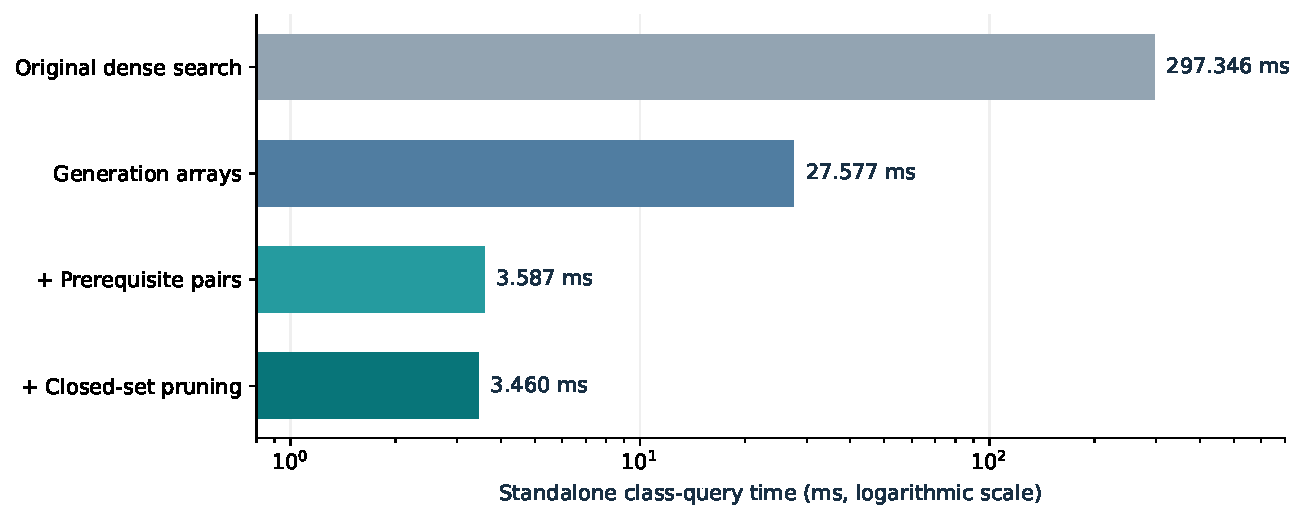
\includegraphics[width=.94\textwidth]{figures/seed_ablation.pdf}
\caption{Measured Gordian two-seed class query. The logarithmic horizontal
scale separates the reusable-state gain from the candidate-set theorem.
This figure does not report whole-knot recognition time.}
\end{figure}

\subsection{Whole-pipeline results and negative cases}

The 800 measured whole-pipeline calls contain 780 completed verdicts,
all equal to the established corpus label, and twenty censored ordinary
Gordian calls that return \code{UNKNOWN}. A timeout is not assigned an
artificial finite speedup.

For survivor-00, the ordinary option set has baseline and new medians
1.950 and 1.690 milliseconds and a median matched speedup of 1.221.
With compressed group search enabled, the corresponding medians are
1.968 and 1.580 milliseconds and the matched speedup is 1.245.

For Gordian with compressed group search, the matched ratio is only
1.034; the separately measured medians are 1.338 seconds for the baseline
and 1.375 seconds for the changed version. Their different ordering is
possible because the median of ratios and the ratio of medians are
different statistics. It illustrates why this small whole-query change
must not be described as a robust universal speedup. The subsequent
roughly 1.3-second recognizer dominates the saved seed work. The ordinary
Gordian configuration never finishes within its cap in either version.

Several small standalone cases regress, including trefoil, figure-eight
and survivor-11; the complete table and A/A controls retain those results.
The stage remains opt-in. The measurements support an exact search
improvement with a large local gain on sparse failures, not a blanket
improvement on every recognized knot.

\subsection{Native compressed surface scaling}
The layered-solid-torus family is inherited from the preceding reports.
Its supplied meridian vector has Fibonacci growth; no claim of a new family is made.
Each measured vector is certified as one orientable disc with one essential boundary circle.
The following timings use three shuffled rounds, with raw samples retained.
\begin{center}\small\begin{tabular}{@{}rrrrrr@{}}
\toprule $t$ & Disc-count bits & Count ms & Proof ms & Replay ms & Proof KiB\\\midrule
1 & 2 & 0.368 & 0.365 & 0.316 & 3.7\\
4 & 5 & 3.564 & 3.951 & 1.585 & 29.8\\
8 & 8 & 12.886 & 13.315 & 3.783 & 87.8\\
12 & 11 & 29.744 & 30.479 & 7.281 & 169.1\\
16 & 14 & 80.155 & 82.503 & 18.313 & 274.1\\
32 & 25 & 225.174 & 265.364 & 34.092 & 938.4\\
64 & 47 & 1310.748 & 1516.839 & 188.950 & 3446.5\\
128 & 92 & 8045.830 & 8103.743 & 628.618 & 13188.4\\
\bottomrule\end{tabular}\end{center}
At $t=128$, the input has 384 nonempty stacks, 764 surface face bands, and
\[N=2\,791\,715\,456\,571\,051\,233\,611\,642\,548\]
normal discs. The ordinary orbit query needs 390 cycles and 41,643 transmissions;
its orientation lift needs 779 cycles. These are algorithmic counts, not sheet counts.
The full five-query certificate occupies 13,504,926 bytes as compact JSON.
The size is charged explicitly; binary geometry does not make certificate transport free.

\begin{figure}[ht]\centering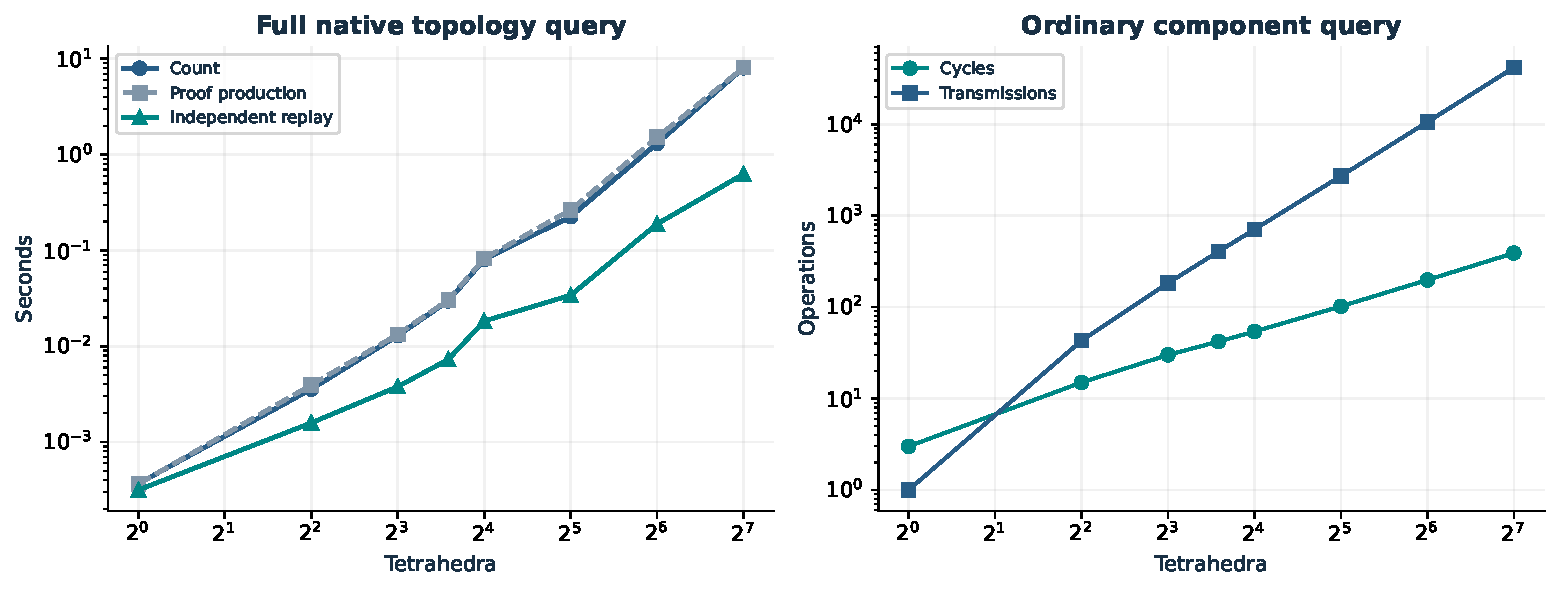
\includegraphics[width=\textwidth]{figures/normal_scaling.pdf}
\caption{Measured native topology costs and ordinary orbit work on supplied Fibonacci
meridian vectors. Lines join measured points only. They are not a fitted universal
complexity law.}\end{figure}

The small explicit controls are often faster. At $t=12$, literal polygon assembly
takes 9.659 ms versus 29.744 ms for the new aggregate query; Regina's component
routine takes 0.906 ms. At $t=16$, the literal control takes 98.205 ms versus
80.155 ms, while Regina remains faster at 3.226 ms. Those controls return a
different output protocol, and these figures are not claimed as certificate-level speedups.
Both explicit controls are restricted to at most 20,000 discs in the final benchmark.
Regina's documented \code{components()} routine explicitly constructs normal discs
\cite{reginadoc}; an initial uncapped diagnostic reached the 64-tetrahedron case
and raised \code{MemoryError: std::bad\_alloc}. Its aborted log is retained separately
and contributes no primary timing ratio. We then applied the same finite-oracle
cap to both explicit controls and reran the complete source-guarded benchmark.
The large rows therefore establish native compressed completion and proof replay,
not a fabricated ratio against a censored explicit computation.


\subsection{Port-incidence costs and the output contract}

For the family $N=7\cdot2^{4096}$, the primary pairings identify residues
modulo $2^{4096}$ and the selected ports are supplied unions of intervals.
The measured medians are:
\begin{center}
\begin{tabular}{@{}rrrrr@{}}
\toprule Ports & Histogram slots & Count (ms) & Proof (ms) & Replay (ms)\\\midrule
2 & 4 & 0.232 & 0.253 & 0.214\\
4 & 16 & 1.761 & 1.625 & 1.313\\
6 & 64 & 8.867 & 9.911 & 7.780\\
8 & 256 & 48.168 & 54.247 & 40.698\\\bottomrule
\end{tabular}
\end{center}
The eight-port proof serializes to 13,866,578 bytes in compact JSON.
This cost is recorded and charged even though the mathematical output
has only 256 integer slots. Only the selected 1,024-bit four-port proof
is retained as a separate replay fixture; the larger proof's size and
digest are in the data. Count-only mode does not retain those traces.

The small-universe comparison supplies an important counterweight. For
$N=7\cdot2^{12}$ and eight ports, the new method takes 25.059 milliseconds
versus 10.355 milliseconds for literal enumeration. With two ports at the
same size, it takes 0.151 milliseconds versus 8.517 milliseconds. Avoiding
sheet expansion does not automatically win when the expanded instance
is small and the number of coned queries is large.

These are generic queries on supplied interval systems. They are not
whole-recognizer timings, not a benchmark against the weighted AHT
algorithm, and not evidence that all geometric attachment information
has been recovered.

\subsection{An inherited worker failure repaired separately}

The first full regression run executed 833 tests and reproduced one
existing failure in the optional normal-surface subprocess wrapper. A
500,000-character request was not completely transmitted when a timed
\code{communicate} call was retried with no input on this Python version.
This defect predates the interval and seed changes and had already been
identified in incoming reports; the maintained baseline still contained
the failing path.

The focused repair gives one worker thread ownership of a single
\code{communicate(payload)} call while the main thread polls its future
for cancellation and deadline handling. On exit the child is killed
when necessary, reaped, the communication owner is joined, and the pipes
are closed. The existing eight worker tests pass, including delayed
large-input transmission, local timeout, global cancellation, and
actual Regina verdicts. This is an engineering repair, not one of the
mathematical advances. The seed benchmark does not import this worker
path, so its measured dependency hashes remain unchanged.

\subsection{Interpretation of the evidence}

The strongest experimental conclusion is agreement across independent
representations, coupled with successful processing of genuine normal
vectors whose disc multiplicity is far beyond enumeration. The strongest
search improvement is the reduction from a quadratic candidate set to
a linear one under a checked hypothesis, combined with output-sensitive
closure work. The data show where each matters and where it does not.
None of the experiments estimates a universal hierarchy depth or proves
the missing complete recognition bound.


\section{Where the quasi-polynomial argument still stops}
\label{sec:gap}

\subsection{An end-to-end accounting statement}

Suppose a recognition procedure executes $R(n)$ hierarchy transitions. Let
$H(n)$ bound the total encoded input size of one transition, including
normal coordinates, residual handles, marks and attaching data, and let
$r(n)$ bound the number of ports whenever the full incidence histogram is
requested. The new local operations contribute at most
\[
 R(n)\,2^{O(r(n))}\poly(H(n))
\]
bit operations, with the $2^r$ factor omitted where ordinary topology
counts suffice. This is an accounting lemma: it follows by summing actual
transition costs, including verification if required.

Consequently, polynomial $H(n)$ together with
\[
 \log R(n)+r(n)=O((\log n)^2)
\]
would place these implemented operations within a quasi-polynomial budget.
This conclusion also requires all other transition operations to have the
same bound and the overall procedure to be sound and complete. The local
theorems provide no bound on $R,H$ or $r$ for arbitrary knot diagrams.

\subsection{Hierarchy resets remain a global issue}

In Lackenby's Section 9 accounting, a hierarchy of maximum length $L$
and maximum pattern complexity $g$ has an iteration bound of the form
\[
 L(g+1)^L.
\]
An efficient representation of one cut does not imply $L=O(\log n)$,
nor does it control the work of reconstructing later surfaces after an
earlier surface is simplified. Repeatedly discarding and rebuilding
suffixes can dominate a locally polynomial operation.

The 2021 talk outlines additional geometric mechanisms aimed at a
logarithmic effective depth \cite{slides}. The present code does not
implement and prove the full hierarchical multi-surface, Cheeger-region,
weak-reduction and reset machinery. The 2026 paper's compressed-cutting
theorem is relevant infrastructure, but its existence cannot be substituted
for the missing implementation and global accounting.

\subsection{Verification does not find a certificate}

The normal-disc input may have exponentially large numerical coordinates
but polynomial bit size. We now verify that input natively in polynomial
bit time. We have not shown that the producer can find a suitable disc
within the same budget. This is the familiar difference between a compact
witness and an efficient deterministic decision algorithm.

Similarly, the port histogram avoids enumerating individual sheets, but
requesting exponentially many distinct port subsets still has a cost.
The result does not eliminate a search over incompatible surface choices
or preserve every attachment datum required by the next transition.

\subsection{The algebraic fallback remains necessary}

The two-seed theorem decides a useful supplied-diagram condition. It does
not bound the seed number of an arbitrary unknot diagram, produce a short
Reidemeister or Markov path to that class, or control the size of an
explicit Khovanov complex. Neither local interval compression nor a
successful seed-search optimization supplies such a bound. The exact
recognizer's fallback is therefore retained, and its general worst-case
complexity remains unchanged by this delivery.

\section{Proposed research program}
\label{sec:future}

The next steps should be judged by a checked input/output contract and a
measured or proved bottleneck reduction. The following priorities follow
directly from the new capability.

\begin{enumerate}[label=\textbf{\arabic*.},itemsep=6pt]
\item \textbf{Weighted general interval orbits.}
Implement the AHT weight transport while retaining independent local
certificates. The target is a compressed collection of per-component
normal-coordinate and Euler data. Validate against the native topology
summary and full Regina component vectors. A satisfactory implementation
must handle many identical components without printing one record per
sheet and must include integer-weight growth in its cost.

\item \textbf{Boundary order and attachment words.}
Extend the port histogram to preserve cyclic order or a compressed
boundary permutation. Identify exactly which hierarchy decisions need
more than a set-valued signature. Success means a consumer can reconstruct
and check a specified gluing operation; matching aggregate counts alone
is insufficient.

\item \textbf{A checked PD-to-exterior-to-disc pipeline.}
Produce a triangulated exterior with a replayable combinatorial link to
the original diagram, obtain a normal disc vector from a search engine,
and verify it with the native certificate. This would convert an external
positive verdict into a bound-to-input certificate. It must retain
manifold and peripheral provenance through simplification.

\item \textbf{Complete residual-cell attachments after cutting.}
Combine the imported extractor's bounded residual cells and prism bands
with general interval topology. Recover the attachment of every vertical
boundary annulus or square to those cells, including edge-neighborhood
cleanup. Test reconstructed complements, not just counts, on triangulations
where a separate engine can explicitly cut.

\item \textbf{Reduce the polynomial overhead of the general orbit engine.}
Profile failed periodic-merger scans, maximal-pairing selection and
certificate transport. Replace repeated quadratic scans by a proved
index or event structure. Preserve the same small local checker. A useful
result should improve the complete topology query on the layered torus
family and on mixed/nonorientable data, with count-only and certified
modes reported separately.

\item \textbf{Sparse seed search beyond trivial singleton closures.}
Study the family of singleton closures before selecting a second seed.
The first interaction between two such closures must cross a binary
prerequisite. Can an incidence index enumerate all potentially successful
pairs output-sensitively while preserving the lexicographic first witness?
A proof must account for large overlapping singleton closures rather
than assuming the sparse case persists after reduction.

\item \textbf{Short certificates for two-seed failure.}
The current negative result is exhaustive search over a checked candidate
graph. A family of proper closed sets covering all candidate edges would
be a compact nonmembership witness for the derivation class. Investigate
minimum or approximate covers and verify them without closure searches.
This still certifies a diagram property, not knottedness.

\item \textbf{A global hierarchy potential that survives resets.}
Track encoded handle size, attachment complexity, surface bit lengths
and the cost of rebuilding discarded suffixes in one potential. Prove a
bound on total transition work, rather than independent local bounds.
This is the main missing step toward an unrestricted quasi-polynomial
recognizer.

\item \textbf{Certificate-level formalization.}
Formalize the six interval proof rules, coning identity, Boolean inversion,
orientation-cover formulas and prerequisite-pair theorem in Lean. These
are finite combinatorial statements with small interfaces. The initial
goal should be a verified checker specification; formalizing all of
normal-surface topology at once would obscure this tractable boundary.
\end{enumerate}

\section{Reproduction, integration, and deliverable boundaries}
\label{sec:reproduce}

The ZIP contains this article and its PDF, the modified runnable Python
package, new tests and experiments, raw results, a patch against the pinned
commit, provenance notes, and checksums. Third-party papers and unrelated
historical archives are not needed to run the new code.

From the delivered \path{snapshot/Topology/UnknotRecognition/fast} directory:
\begin{lstlisting}
python -B -m unittest discover -s tests -v
python -B -m fastunknot.normal_components normal_orbit_research/examples/meridian.json --certificate
python -B normal_orbit_research/validate_normal_orbits.py --native --output results/native_orbit_validation.json
python -B benchmark_two_meridian_search.py --help
python -B benchmark_interval_incidence.py --help
python -B benchmark_normal_orbits.py --help
\end{lstlisting}
The validation driver documents its optional Regina dependency. The orbit
producer, checker, normal summary, seed optimization and their ordinary
unit tests use the Python standard library. The inherited optional native
recognizer is still an independent pipeline option.

The existing extractor is copied from the preceding affine-families
delivery without changes, and its prior tests are retained. New files are
kept small enough to review separately: the interval producer, interval
verifier, normal adapter and incidence module have distinct responsibilities.
The optimized two-meridian search preserves the old dense propagation
routine as a reference oracle, while a frozen baseline module supports
the measured historical comparison.

The delivered patch is intended for review and integration. It does not
publish a branch, create a pull request, or alter the user's remote
repository. The standalone article does not overwrite the project's large
maintained synthesis manuscript; the integration notes explain where its
new section can be incorporated.

\appendix
\section{Mathematical and experimental claim ledger}

\begin{longtable}{@{}p{.29\textwidth}p{.19\textwidth}p{.45\textwidth}@{}}
\toprule Claim & Status & Exact qualification\\\midrule\endhead
Polynomial interval orbit counting & Classical theorem, implemented &
AHT, arbitrary partial isometries; no sheet expansion\\
Local trace soundness & Proved and tested &
Checker binds initial system; complete trace required\\
Marked-union coning formula & Proved &
Counts touched orbits, not marked points\\
$2^r$ port histogram & Proved and implemented &
Complete set-incidence histogram; no boundary order or attaching words\\
Polynomial native normal summary & Proved under explicit input conditions &
Valid compact ambient manifold and embedded admissible normal surface\\
Compressing-disc certificate & Proved sufficient &
Positive mod-two boundary test; torus case exact for one simple curve\\
Knot verdict from supplied triangulation & Conditional &
Requires separately checked $S^3$ knot-exterior provenance\\
At most $2n$ pair candidates & Proved on checked class &
Trivial singleton closures; productive-unary systems use complete fallback\\
Quadratic seed-search work & Proved on checked class &
Excludes subsequent integer arithmetic and earlier pipeline filters\\
Natural-diagram speed changes & Measured &
Paired controls, exact workload and resource policy recorded in raw data\\
General $\qp$ recognition & Unproved &
Encoded-size, surface-search, attachment, depth and reset obligations remain\\
\bottomrule
\end{longtable}

\section{Reference interfaces}

\begin{lstlisting}[language=Python]
from fastunknot.interval_orbits import analyze_orbits
from fastunknot.interval_orbit_verify import verify_orbit_certificate

maps = [{"start": 0, "stop": 80, "sign": 1, "offset": 20}]
answer = analyze_orbits(100, maps, record_trace=True)
assert answer["orbit_count"] == 20
assert verify_orbit_certificate(100, maps, answer["certificate"])

from fastunknot.normal_components import (
    analyze_normal_surface, verify_normal_surface_certificate,
)
answer = analyze_normal_surface(triangulation, coordinates,
                                record_trace=True)
assert verify_normal_surface_certificate(
    triangulation, coordinates, answer["certificate"])
\end{lstlisting}

The normal input uses actual tetrahedral permutations and normal
coordinates, not a guessed global cyclic-cover description. Large integers
in JSON may use exact hexadecimal strings. A false certificate-verification
result rejects the stated evidence. Invalid ambient-input schemas can raise
an extraction error; caller cancellation is deliberately propagated.

\begin{thebibliography}{20}
\bibitem{aht}
I.~Agol, J.~Hass, and W.~P.~Thurston,
\emph{The computational complexity of knot genus and spanning area}.
\href{https://arxiv.org/abs/math/0205057v2}{arXiv:math/0205057v2},
revised 10 July 2004; especially Sections 4 and 6.

\bibitem{lackenby2026}
M.~Lackenby,
\emph{Incompressible surfaces, hierarchies and unknot recognition}.
\href{https://arxiv.org/abs/2607.23350}{arXiv:2607.23350v1}, 25 July 2026;
especially Section 9 and Theorem 14.4.

\bibitem{slides}
M.~Lackenby, \emph{Unknot recognition in quasi-polynomial time},
lecture slides, 2021.
\url{https://people.maths.ox.ac.uk/lackenby/quasipolynomial-talk.pdf}.

\bibitem{proveit}
V.~Reshetnikov and contributors, \emph{ProveIt: Topology/UnknotRecognition},
pinned revision \texttt{2b93767bd3cf7ea7c1995acd66f50c72858a30c5},
accessed 8 October 2026.
\url{https://github.com/VladimirReshetnikov/ProveIt/tree/2b93767bd3cf7ea7c1995acd66f50c72858a30c5/Topology/UnknotRecognition}.

\bibitem{affine}
ProveIt research continuation, \emph{Affine families}, 8 October 2026.
Incoming archive \path{docs/incoming/unknot_affine_families_20261008.zip}
and maintained review \path{synthesis/affine_families_review.tex} in
\cite{proveit}. Source of the unchanged normal-interval extractor and
layered-torus test fixtures used here.

\bibitem{twomeridian}
ProveIt contributors, \emph{Checked two-meridian recognition},
\path{synthesis/two_meridian.tex} and \path{fast/fastunknot/two_meridian.py}
in \cite{proveit}. Source of the retained arithmetic and positive
certificate contract.

\bibitem{regina}
B.~A.~Burton and the Regina developers, \emph{Regina: software for
low-dimensional topology}. \url{https://regina-normal.github.io/}.
Version used by the experiments is recorded with their results.

\bibitem{reginadoc}
Regina developers, \emph{NormalSurface class reference},
documentation of \code{components()}, accessed 8 October 2026.
\url{https://regina-normal.github.io/engine-docs/classregina_1_1NormalSurface.html}.
\end{thebibliography}
\end{document}
